\documentclass[a4paper, 11pt]{article}

%% packages
\usepackage{fullpage} % changes the margin
\usepackage{hyperref} % Links
\usepackage[utf8]{inputenc}
\usepackage{lmodern}
\usepackage{amsfonts}
\usepackage{amsthm}
\usepackage{amsmath}
\usepackage{braket}
\usepackage{graphicx}
%%

%% environments
\theoremstyle{definition}
\newtheorem{definition}{Definition}
\newtheorem{examples}{Example}
\newtheorem{exercises}{Exercises}
\newtheorem{exercise}{Exercise}
\newtheorem{postulate}{Postulate}
%%

%% config
\date{}
\linespread{1.15}
%%

\begin{document}

\allowdisplaybreaks[2]
\title{Quantum Computing @ MEF \\ \small{TPC-1}}
\author{Renato Neves \\ \scriptsize
  \href{mailto:nevrenato@di.uminho.pt}{nevrenato@di.uminho.pt}}
\maketitle

\noindent
Figure~\ref{fig:qt} presents the circuit respective to quantum
teleportation. Analyse this circuit and then solve the two exercises
below.
\begin{figure}[h]
  \centering
  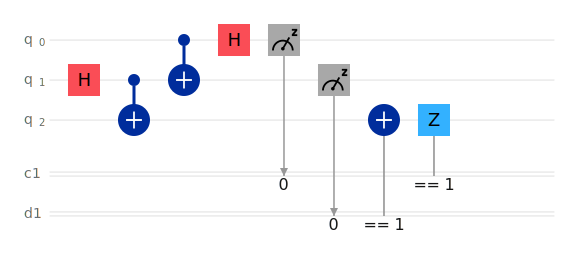
\includegraphics[scale=0.7]{teleport.pdf}
  \caption{Quantum teleportation circuit.}
  \label{fig:qt}
\end{figure}

\noindent
\textbf{Exercise 1.} Write down the mathematical laws and definitions
that were used at each step
in following calculation.
\begin{align*}
  & \left (\alpha \ket{0} + \beta \ket{1} \right ) \otimes \left
  (\frac{1}{\sqrt{2}}\ket{00} + \frac{1}{\sqrt{2}}\ket{11} \right ) \\
  & = \{\ \dots  \} \\
  & = \frac{1}{\sqrt{2}} \big ( \left (\alpha \ket{0} + \beta \ket{1} \right )
    \otimes \left (\ket{00} + \ket{11} \right ) \big ) \\
  & = \{\ \dots\ \} \\
  & = \frac{1}{\sqrt{2}} ( \alpha \ket{000} + \alpha \ket{011} +
    \beta \ket{100} + \beta \ket{111} ) \\
  & \mapsto \{\ \dots\ \} \\
  & = \frac{1}{\sqrt{2}} ( \alpha \ket{000} + \alpha \ket{011} +
    \beta \ket{110} + \beta \ket{101} )  \\
  & = \{\ \dots\ \} \\
  & = \frac{1}{\sqrt{2}} ( \ket{0} \otimes \alpha\ket{00} + \ket{0} \otimes
    \alpha \ket{11} + \ket{1} \otimes \beta \ket{10} + \ket{1} \otimes \beta \ket{01} )
  \\
  & = \{\ \dots\ \} \\
  & = \frac{1}{\sqrt{2}} \big ( \ket{0} \otimes (\alpha\ket{00} + \alpha \ket{11}) +
    \ket{1} \otimes (\beta \ket{10} +  \beta \ket{01}) \big ) \\
  & \mapsto \{\ \dots\ \} \\
  & = \frac{1}{\sqrt{2}} \left ( \frac{1}{\sqrt{2}} (\ket{0} + \ket{1})
    \otimes (\alpha\ket{00} + \alpha \ket{11}) + \frac{1}{\sqrt{2}} (\ket{0} - \ket{1})
    \otimes (\beta \ket{10} +  \beta \ket{01}) \right ) \\
  & = \{\ \dots\ \} \\
  & = \frac{1}{2} \left ( (\ket{0} + \ket{1})
    \otimes (\alpha\ket{00} + \ket{11}) +  (\ket{0} - \ket{1})
    \otimes (\beta \ket{10} +  \beta \ket{01}) \right ) \\
  & = \{\ \dots\ \} \\
  & = \frac{1}{2} \left ( \alpha \ket{000} + \alpha \ket{011} +
    \alpha \ket{100} + \alpha \ket{111} + \beta \ket{010} + \beta \ket{001}
    - \beta \ket{110} - \beta \ket{101} \right ) \\
  & = \{\ \dots\ \} \\
  & = \frac{1}{2} \big ( \ket{00} \otimes (\alpha \ket{0} + \beta \ket{1})
    + \ket{01} \otimes (\beta \ket{0} + \alpha \ket{1}) +
    \ket{10} \otimes (\alpha \ket{0} - \beta \ket{1}) +
    \ket{11} \otimes (-\beta \ket{0}  + \alpha \ket{1} ) \big )
\end{align*}

\noindent
\textbf{Exercise 2.} The quantum teleportation protocol
(Fig.~\ref{fig:qt}) starts by putting the qubits shared by Alice and
Bob in the entangled state $\frac{1}{\sqrt{2}}(\ket{00} + \ket{11})$.
Show that after slight modifications the protocol will work equally
well if these two qubits are put instead in the entangled state
$\frac{1}{\sqrt{2}}(\ket{01} + \ket{10})$. Present the modified
circuit in Qiskit and discuss how you can use the latter to test the
circuit.

%% Bibliography
\bibliographystyle{alpha}
\bibliography{biblio}

\end{document}